\section{Result of the Planning}

Ein großer Teil der Planung eines Projektes spiegelt sich im Pflichtenheft wieder. Dort wird die Anforderungsanalyse festgehalten, Ziele deklariert, sowie Entscheidungen und Produktinformationen niedergeschrieben.

\subsection{Software Development Model}

This section contains information about the Software model choosen based on the Requirements of the Project.
The Principals of the Group, the Customer Requirement and Knowledge about the Project play an important role in choosing the Development Model. Based on the Development Model, the Development team decides its work flow. 

\begin{description}
	\leftskip=0,8cm
	\item[Agile Development Model: SCRUM] The Group choose Scrum because it is an iterative and incremental agile software development framework for managing product development.The duration of each Sprint would be two Weeks. Each Phase of the Software Development would have two Sprints. 
	
	Each Sprint would end with a Presentation by each Working Group about the Developments and Progress during the Sprint. The End of each Phase of the Project would be marked by a working Prototype and a Presentation which would include a summary of the work done by the entire Team. 
	
	\item[Projects specific Adaptation to the Model:] Every person in the Team has multiple roles. Each Group member would be working on both, the Document and the Code.
\end{description} 

\subsubsection{Software Development specific Content}
Since the Group decide for the Agile Development Project, the Milestones need to be stated and agreed upon by the Team. Milestones are the Aim or the expected output of each Development Phase. The also give the Outlook and Perspective of the Performance of the System. They help the Team to specify what all should be completed by which Deadline.

\subsection{Aufwandsabschätzung}
Mit der Aufwandsabschätzung wird versucht, die verschiedenen Teile des Projektes anhand von Aufwands- und Komplexitätskriterien einzuteilen. (siehe Abbildung 1)
\clearpage
\begin{figure}
	\begin{center}
		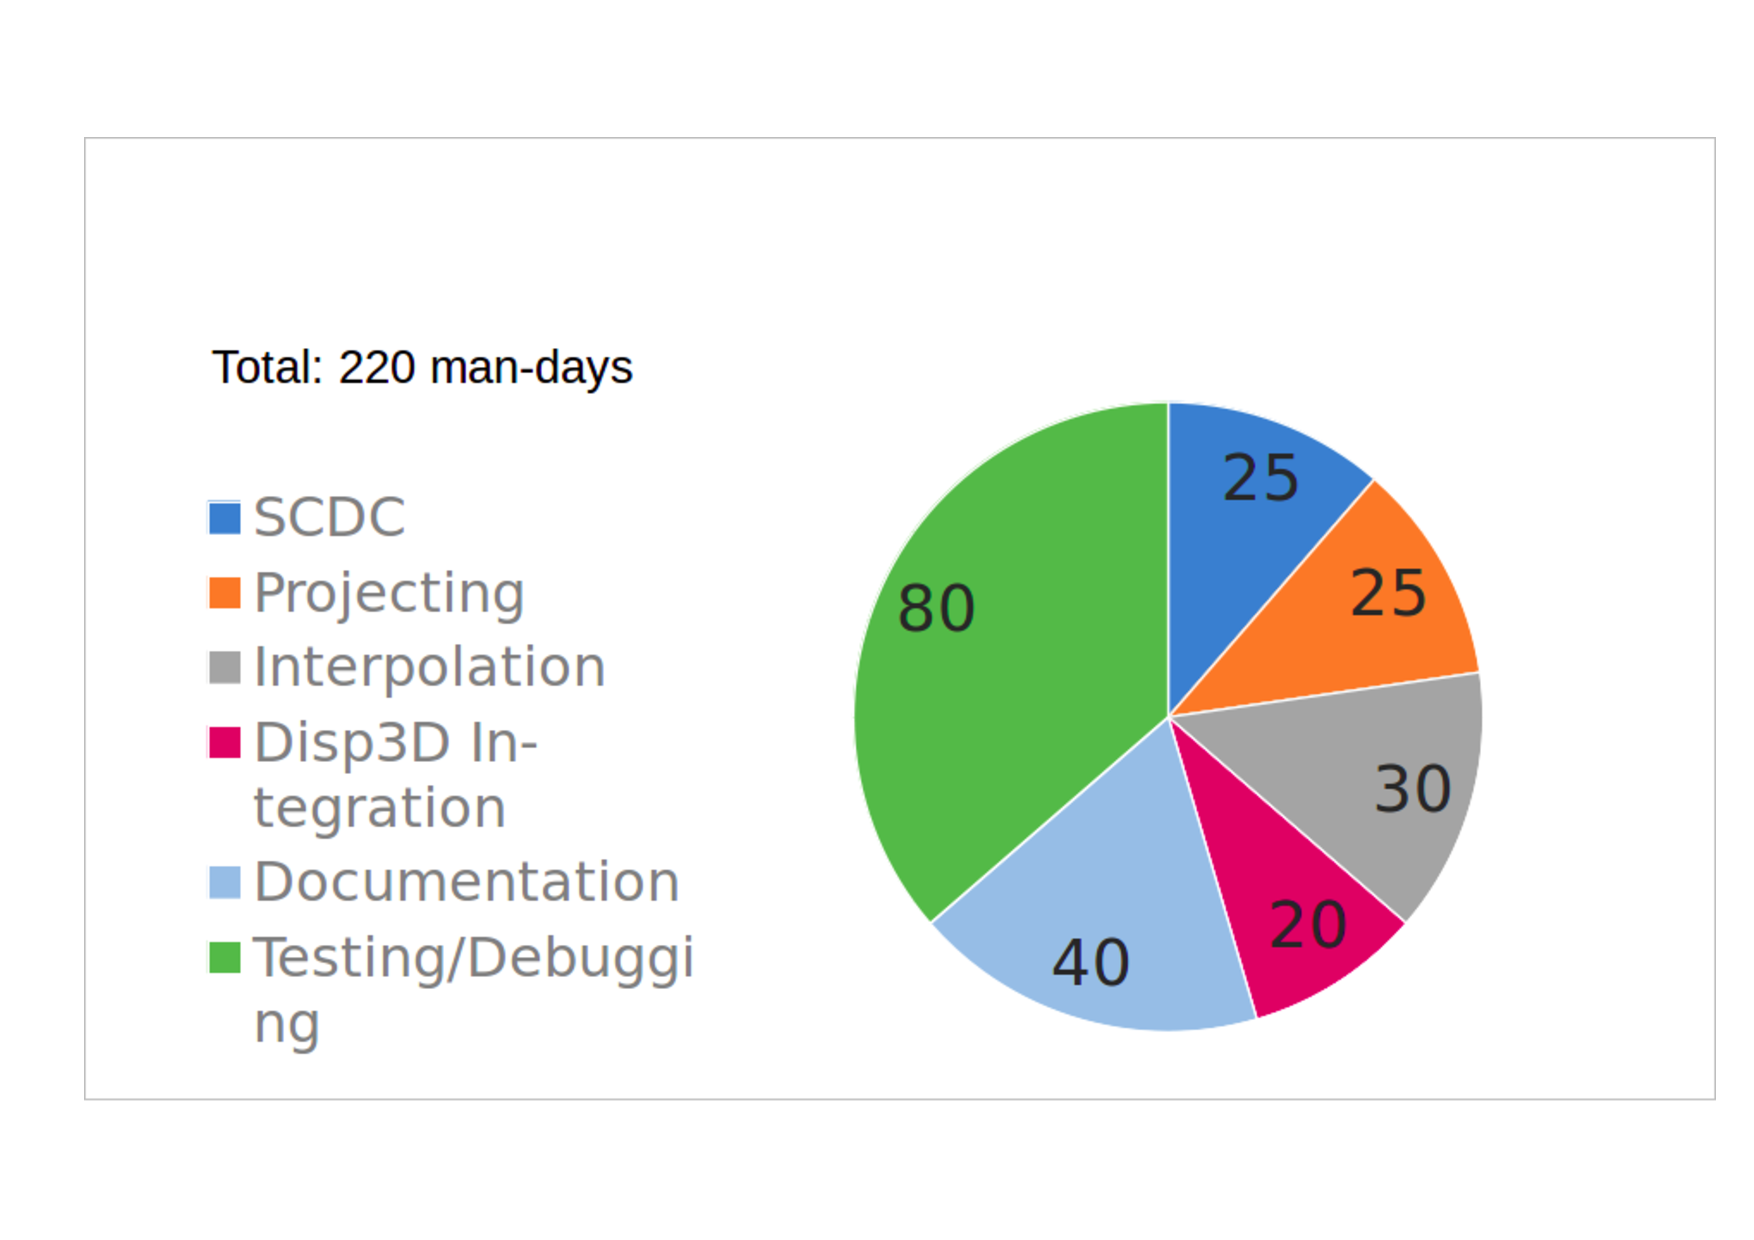
\includegraphics[width= 10cm]{figures/Aufwandsabschaetzung.pdf}
		\caption{Aufwandsabschätzung}
	\end{center}
\end{figure}

\subsection{Risikoabschätzung}
In the following section the Probability of the different Risks involved in the Project are mentioned. The Effect that the potential Risks might cause help determine how important it is for the Team to take care of that Risk and prevent it from occuring.

\begin{figure}
	\begin{center}
		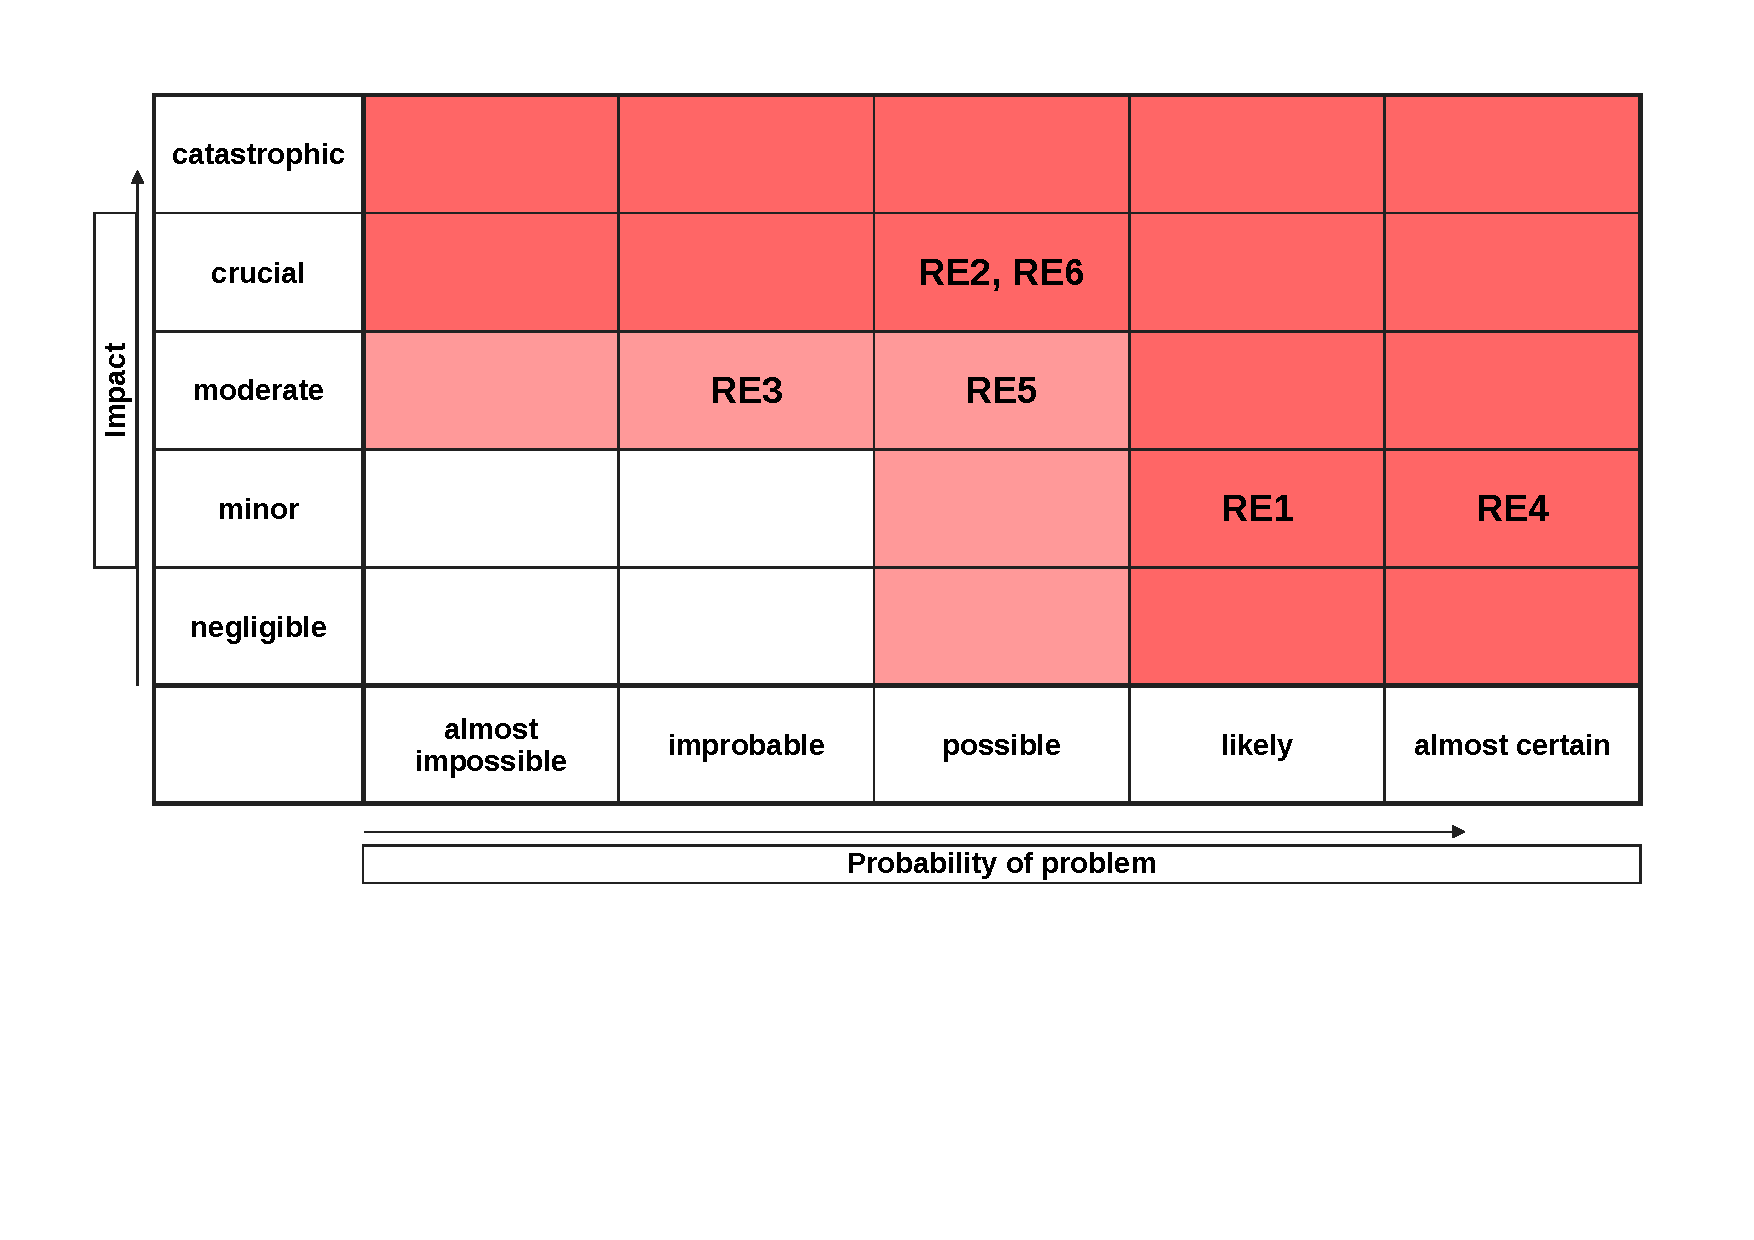
\includegraphics[width= 17cm]{figures/Risikoabschaetzung.pdf}
		\caption{Risikoabschätzung}
	\end{center}
\end{figure}


\begin{description}
	\item[R1:] Kommunikationsprobleme im Team
	\item[R2:] Umfang zu groß
	\item[R3:] Technologie(Rechner) erfüllt nicht die Anforderungen
	\item[R4:] Framework bietet nicht die benötigte Funktionalität
	\item[R5:] Ausfall von Mitgliedern 
	\item[R6:] Anforderungsänderungen durch den Auftraggeber aufgrund eines Kommunikationsproblems im Pflichtenheft
	\item[R7:] falsche Umsetzungsstruktur, gewählte Struktur lässt sich nicht umsetzen
	\item[R8:] Rechtliche Vorgaben
	\item[R9:] versteckte Komplexität
\end{description}

\clearpage

\subsection{Meilensteine}
\begin{description}
	\leftskip=0,8cm
	\item[Erster Meilenstein:] Pflichtenheft, Grobentwurf, lauffähige Implementierung (einfaches Forwarding)
	
	\item[Zweiter Meilenstein:] lauffähige Implementierung (Verschlüsselung mit statischem Schlüssel)
	
	\item[Dritter Meilenstein:] lauffähige Implementierung (Schlüsselaustausch, Gruppenschlüssel), Validierung
\end{description}



\subsection{Organisation}

Die Organisation betrifft alle Regelungen, Vereinbarungen und Aufteilungen der am Projekt beteiligten Personen um ein geordnetes und effizientes Arbeiten zu ermöglichen.

\subsubsection{Kommunikationswege}
\begin{description}
	\item[Zulip:] Dient der schnellen Gruppenkommunikation um effektiv Missverständnisse zu lösen und für eine direkte Kommunikation unter Gruppenmitgliedern.
	
	\item[Email-Verteilerliste:] Dient zur Planung von Treffen und wird für Mitteilungen, die an alle gesendet werden, verwendet.
	
	\item[Gruppentreffen:] Dient zur Diskussion und Besprechung von Problemen. 
	
	\item[Phabricator:] Dient der Zuweisung von Aufgaben an einzelene Gruppenmitglieder und der direkten Kommentierung.
	
\end{description}

\subsubsection{Zusätzliche Vereinbarungen}
\begin{itemize}
	\item Gruppentreffen jeden Donnerstag von 9:00 Uhr - 12:30 Uhr
	
	\item Kleingruppentreffen nach Absprache und Bedarf
	
\end{itemize}

\subsubsection{Rollenverteilung im Agilen Vorgehen}

\begin{description}
	\leftskip=0,8cm
	\item[Produkt Owner:] Michael Rossberg
	
	\item[Scrum Master:] Felix Seidel, Tobias Schubert
	
	\item[Entwicklungsteam:] Felix Seidel, Milan Haverkock, Michael Fuchs, Daniel Scheliga, Yannic Faulwetter, Nils Winkelbach, Jörn Weisensee, Tobias Schubert
	
	\item[Kunde, Anwender:] Telematik Lehrstuhl
	
	\item[Management:] Tobias Schubert
\end{description}

\subsubsection{Organisatorische Rollenverteilung}
\begin{description}
	\leftskip=0,8cm
	\item[Betreuer:] Michael Rossberg
	
	\item[Teamleiter:] Tobias Schubert
	
	\item[Code:] Felix Seidel
	
	\item[Präsentation:] Daniel Scheliga
	
	\item[Grafik:] Nils Winkelbach
	
	\item[Build-Master:] Milan Haverkock
	
	\item[Dokumentation:] Michael Fuchs
	
	\item[Test:] Jörn Weisensee
	
	\item[Web-Master:] Yannic Faulwetter
	
\end{description}

\subsubsection{Programmieraufteilung}
\begin{description}
	\leftskip=0,8cm
	\item[Forwarding]: Milan Haverkock, Daniel Scheliga, Nils Winkelbach
	
	\item[Network]: Felix Seidel, Michael Fuchs, Yannic Faulwetter
	
	\item[Crypto]: Tobias Schubert, Jörn Weisensee
	
	\item[Dispatch]: noch keine genaue Einteilung getroffen
	
	\item[Control]: noch keine genaue Einteilung getroffen
	
	\item[Testing]: noch keine genaue Einteilung getroffen
	
\end{description}

\clearpage